\section{Web Application}
An application was developed using reduced model waveform feature optimizer. Since the optimizer is essentially acts like the backend of a program, creating an application simply meant writing a "front-end".\\
\\
A highly productive python library "streamlit", facilitates with the construction of web applications. Fortunately for the developer, coding in this frame work requires no handling of html elements, and streamlit has tools for acting on important high level data structures, such as the pandas data frame, matplotlib graphs and plotly graphs.\\
\begin{figure}
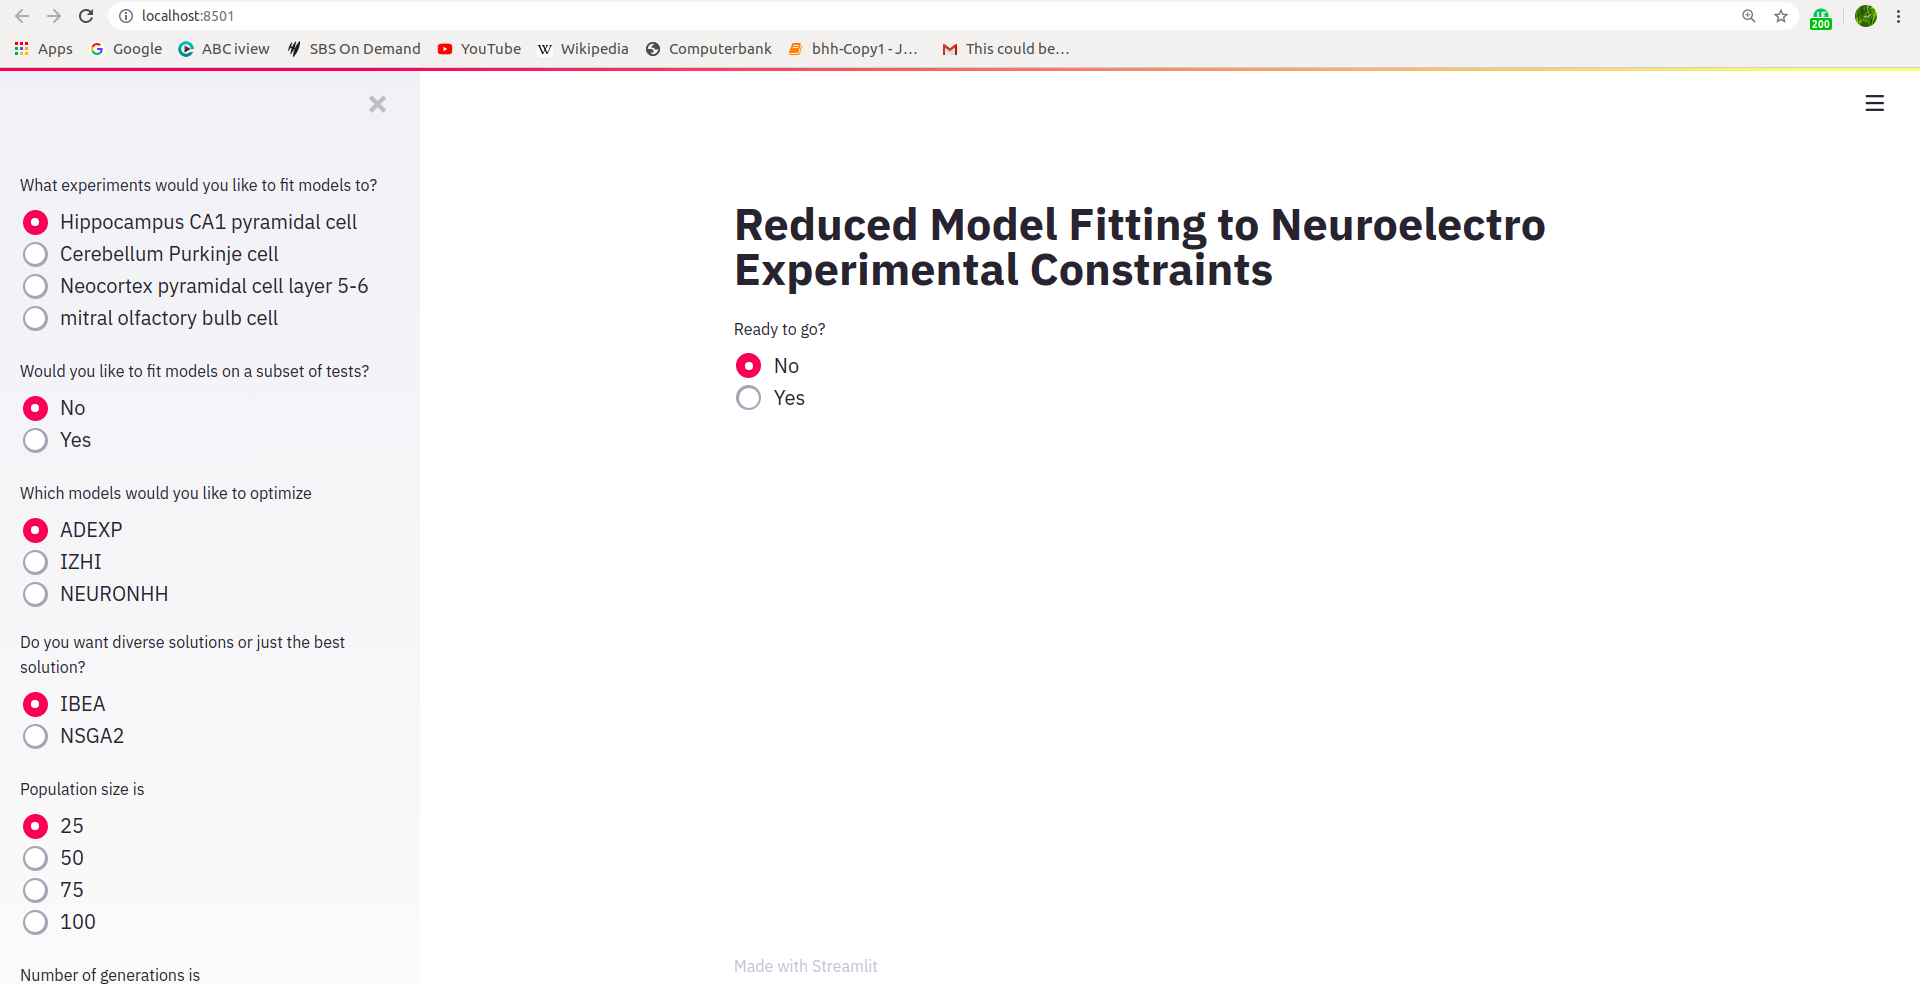
\includegraphics[]{chapters/app_tex/web_app_thesis}
\end{figure}
The side-pane of the web application provides users with a choice of three models, and four data sets that can be used to fit data.
\begin{figure}
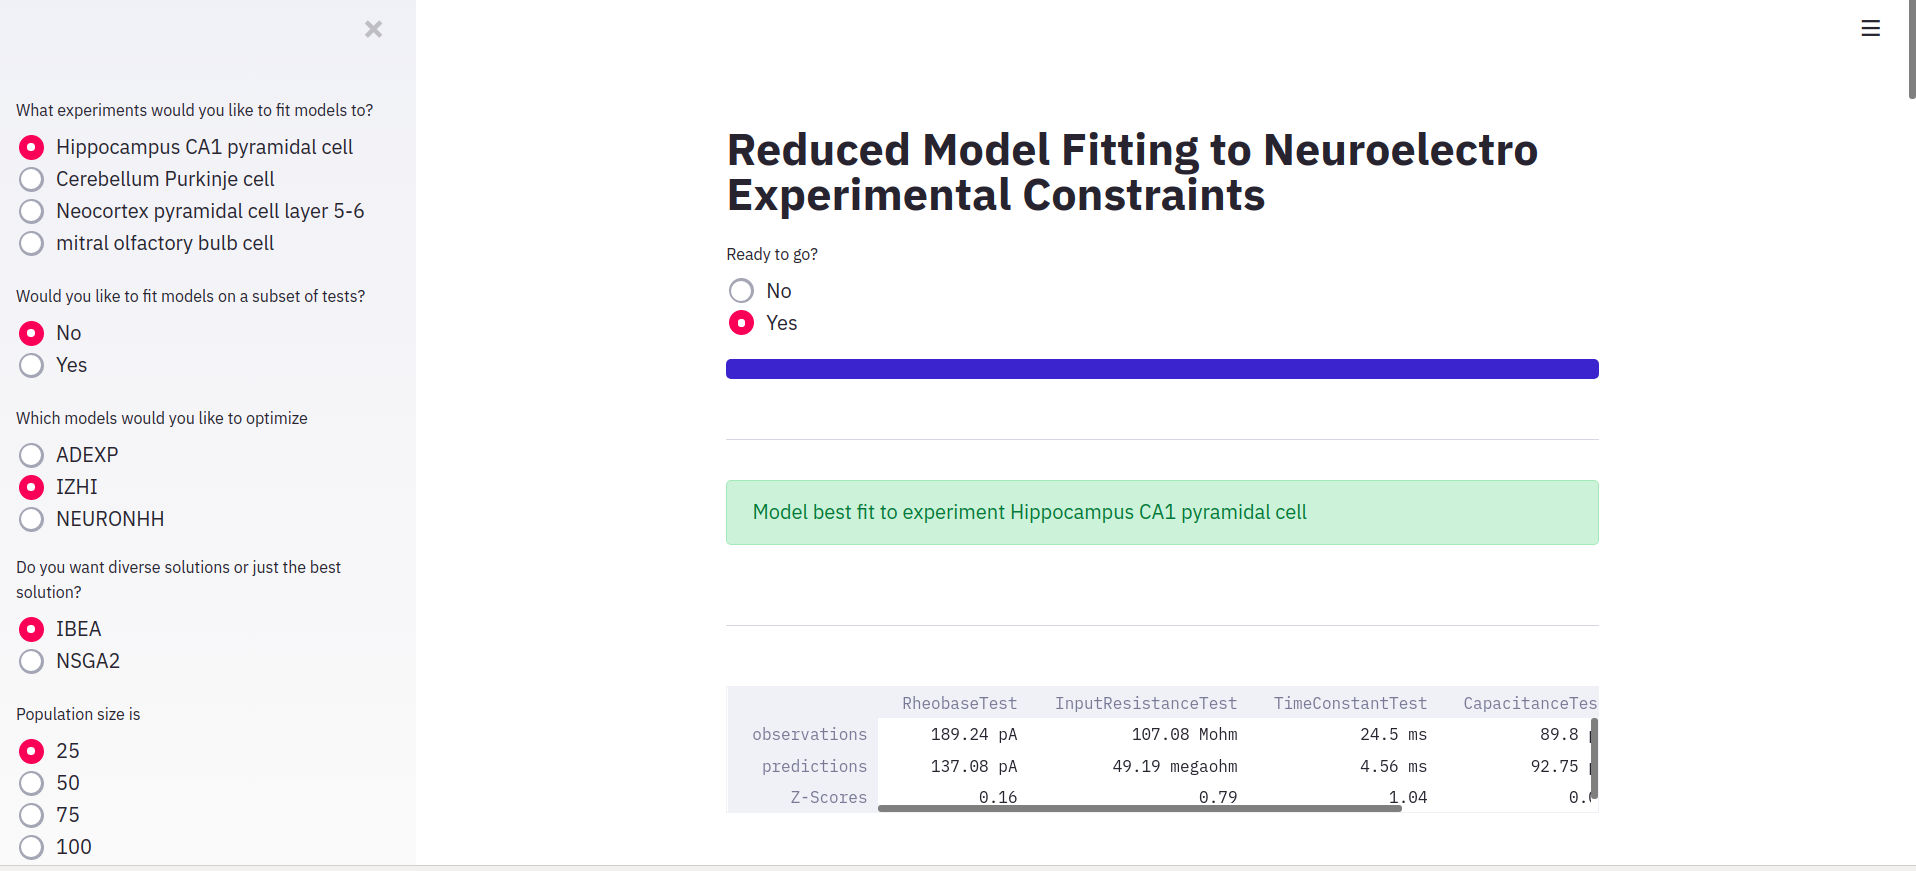
\includegraphics[]{chapters/app_tex/app_results}
\end{figure}

When optimization is complete, the user sees the $\chi^{2}$ statistic, the $p-value$. The user is then allowed to follow a link to download the "model", python object code.\\
\begin{figure}
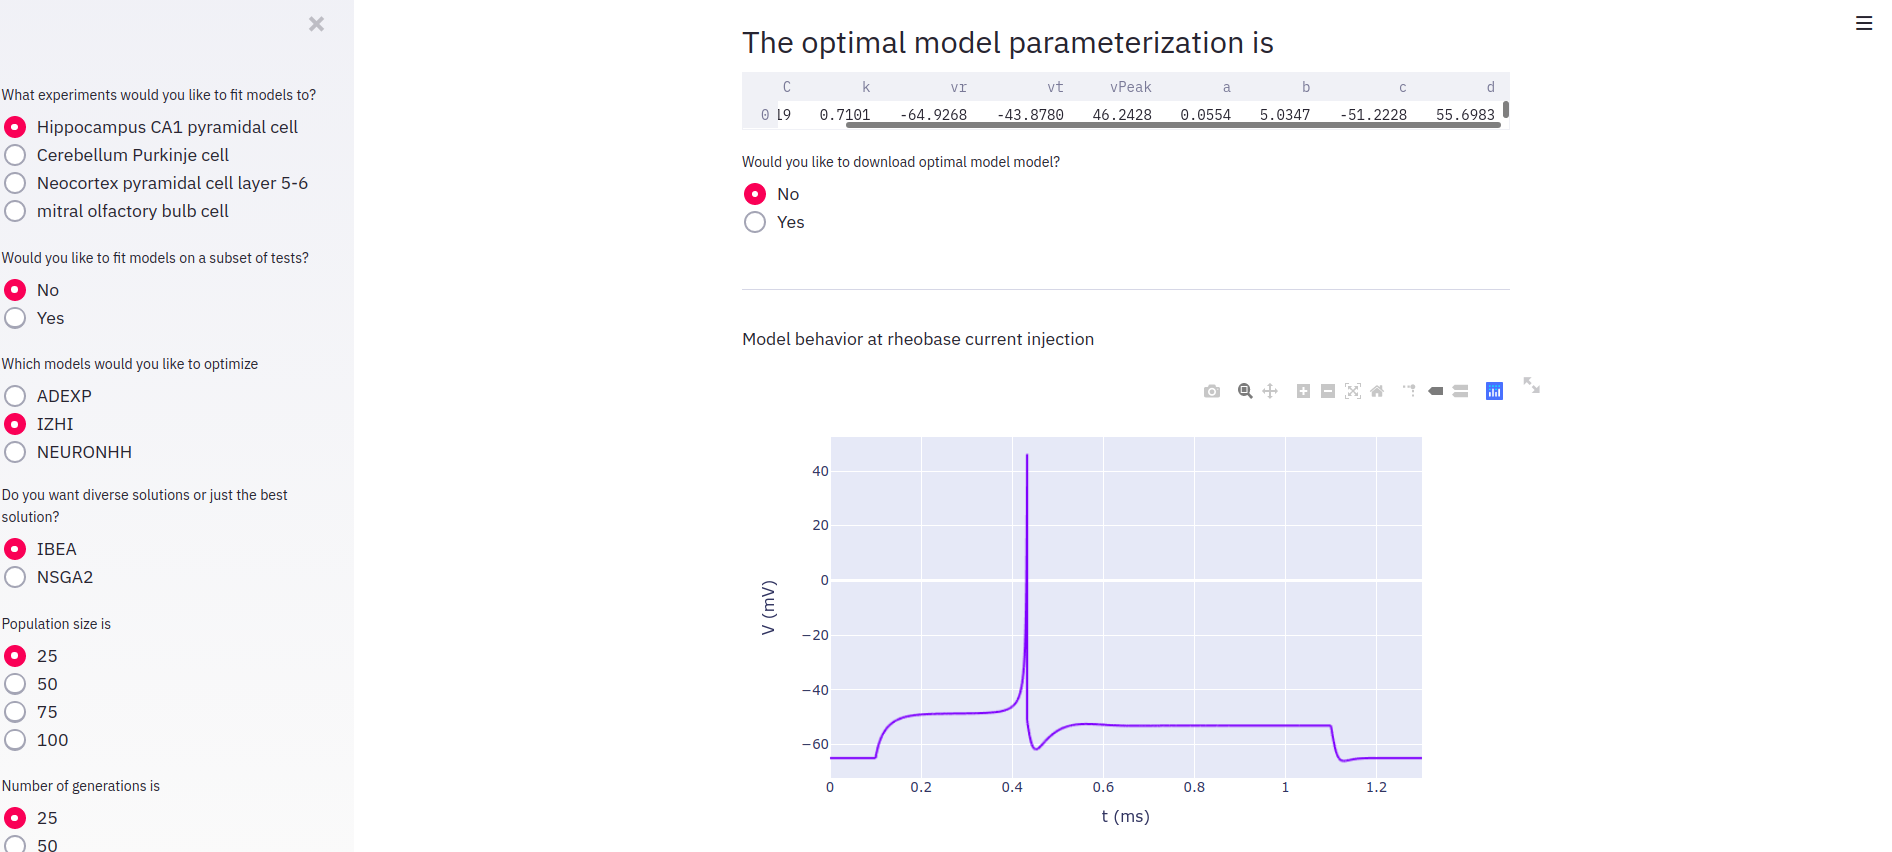
\includegraphics[]{chapters/app_tex/more_app_results}
\end{figure}

An accompanying visualisation of the optimized model neuron firing under rheobase firing, and also under passive conditions is supplied.
\begin{figure}
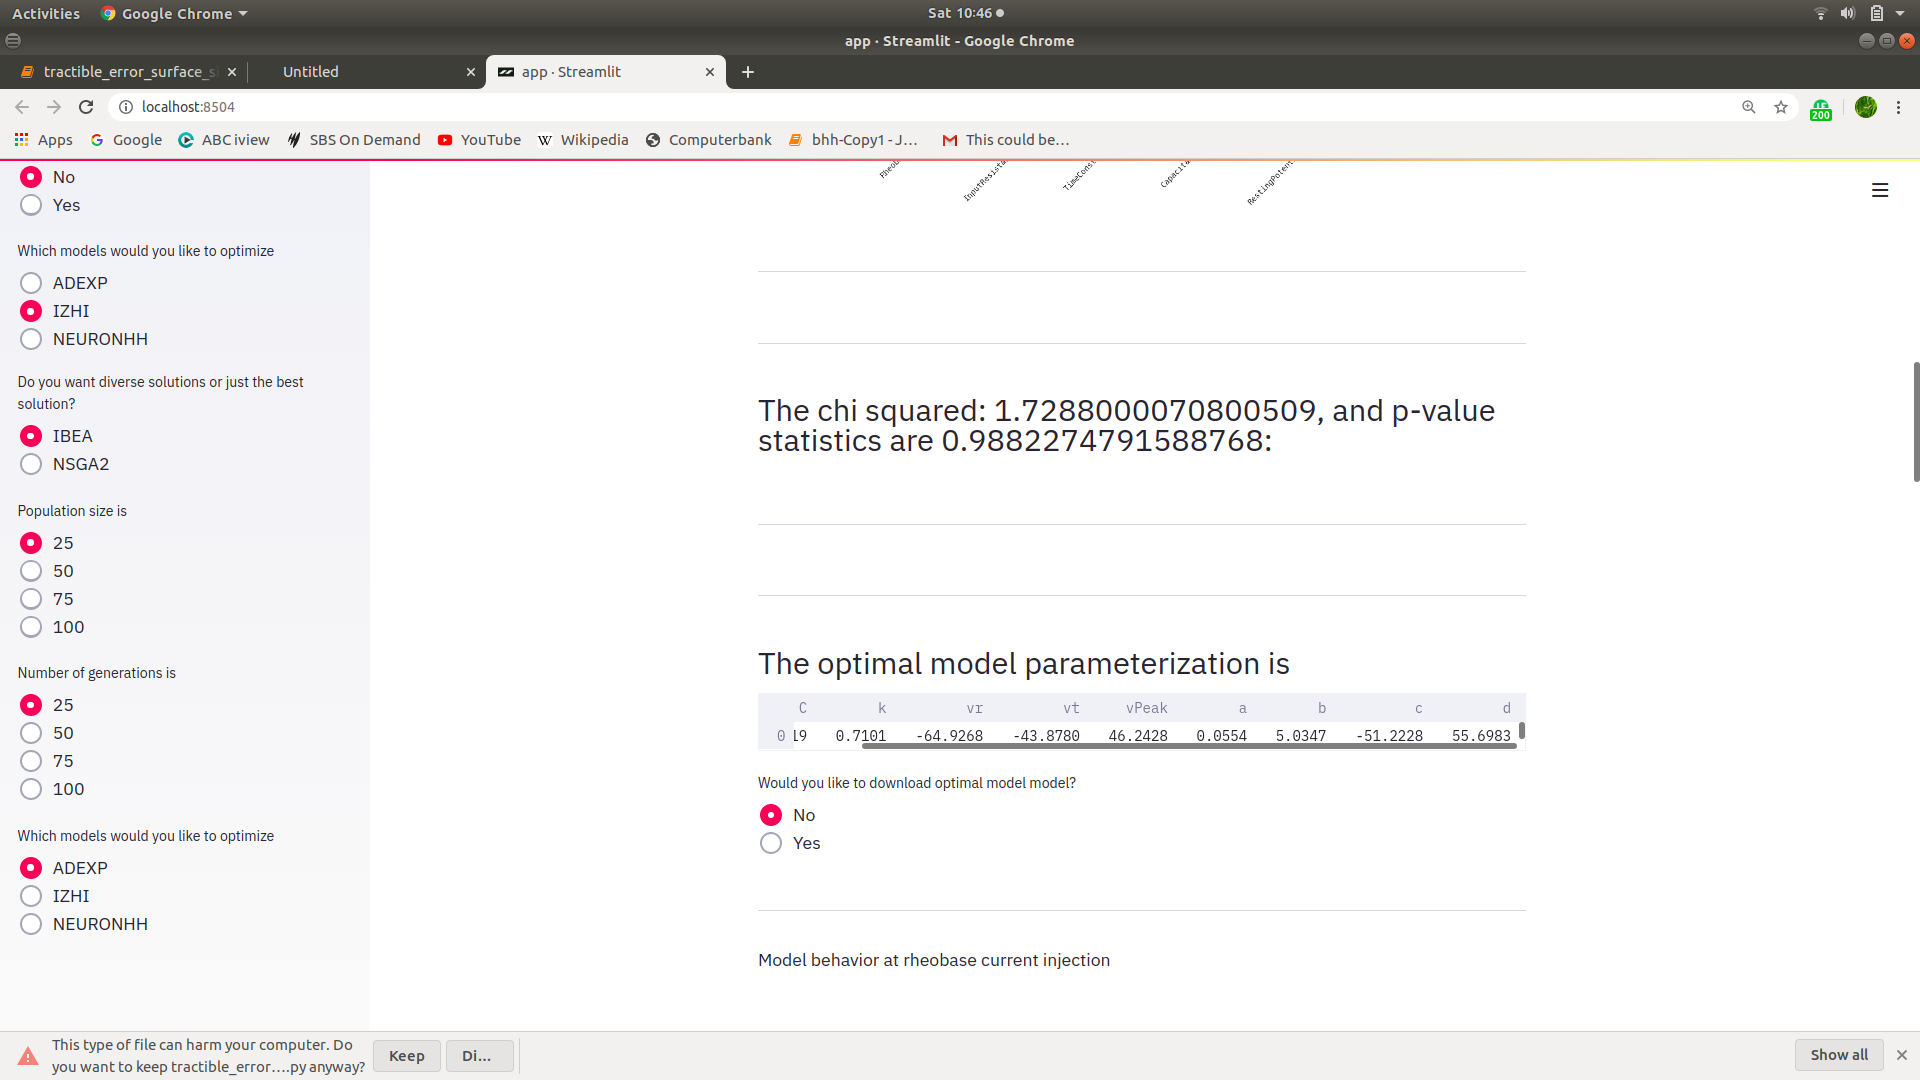
\includegraphics[]{chapters/app_tex/Screenshot from 2020-09-19 10-46-32}
\end{figure}

For each sciunit score in a suite, the Z-scores are visualized as an appropriately placed point on a bell curve. In addition to the $\chi^{2}$ test, this enables users to see how well the model does per test, on features that they may care more about.

The user then has the option of consulting displayed Z-scores, for each test.
\begin{figure}
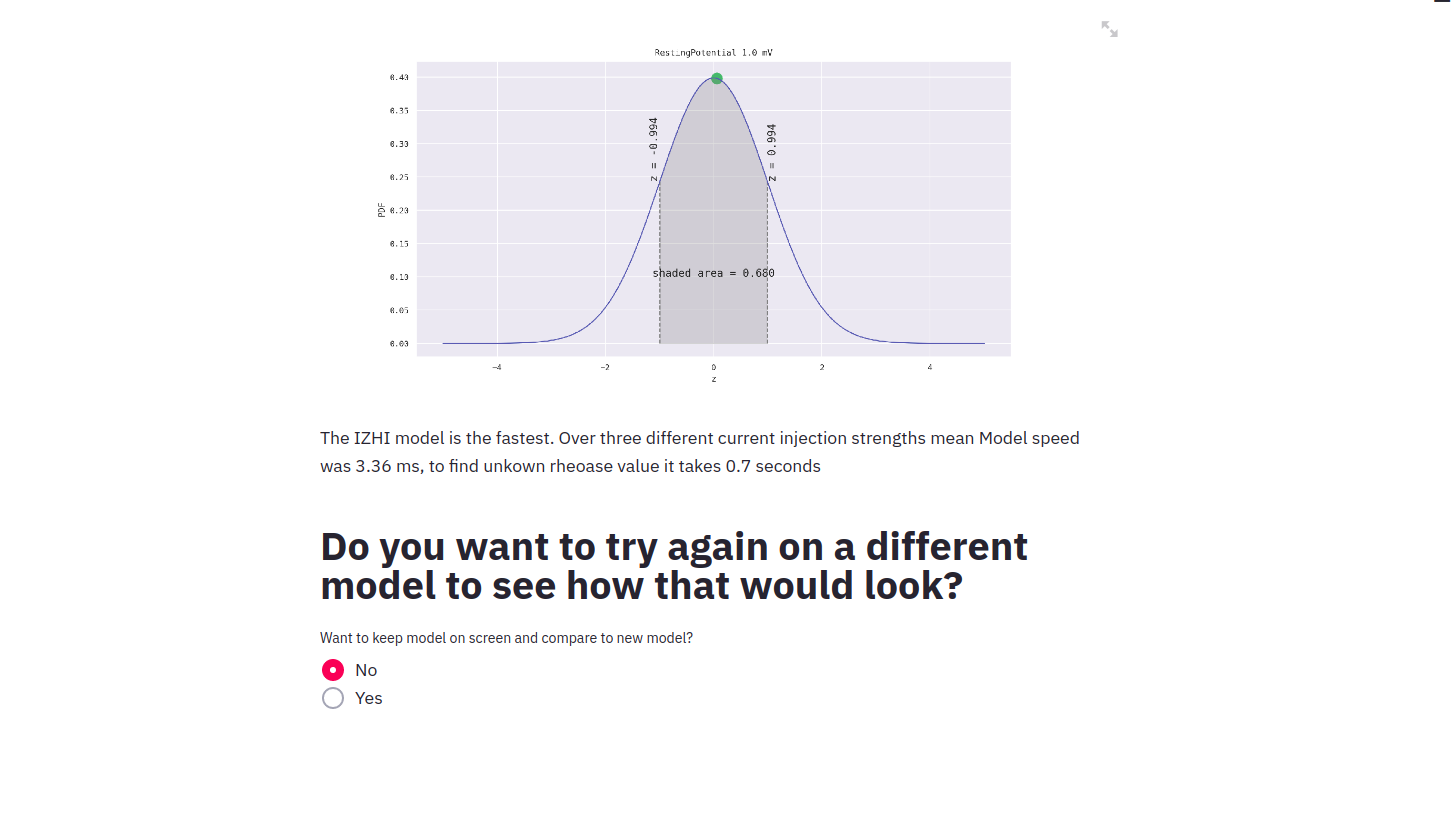
\includegraphics[]{chapters/app_tex/Screenshot from 2020-09-19 10-47-27}
\end{figure}

%\includegraphics[]{chapters/app_tex/Screenshot\ from\ 2020-09-19\ 10-47-31}